\documentclass[12pt, notitlepage, final]{article} 

\newcommand{\name}{Vince Coghlan}

\usepackage{amsfonts}
\usepackage{amssymb}
\usepackage{amsmath}
\usepackage{latexsym}
\usepackage{enumerate}
\usepackage{amsthm}
\usepackage{nccmath}
\usepackage{setspace}
\usepackage[pdftex]{graphicx}
\usepackage{epstopdf}
\usepackage[siunitx]{circuitikz}
\usepackage{tikz}
\usepackage{float}
\usepackage{cancel} 
\usepackage{setspace}
\usepackage{overpic}
\usepackage{mathtools}
\usepackage{listings}
\usepackage{color}

\numberwithin{equation}{section}
\DeclareRobustCommand{\beginProtected}[1]{\begin{#1}}
\DeclareRobustCommand{\endProtected}[1]{\end{#1}}
\newcommand{\dbr}[1]{d_{\mbox{#1BR}}}
\newtheorem{lemma}{Lemma}
\newtheorem*{corollary}{Corollary}
\newtheorem{theorem}{Theorem}
\newtheorem{proposition}{Proposition}
\theoremstyle{definition}
\newtheorem{define}{Definition}
\newcommand{\column}[2]{
\left( \begin{array}{ccc}
#1 \\
#2
\end{array} \right)}

\newdimen\digitwidth
\settowidth\digitwidth{0}
\def~{\hspace{\digitwidth}}

\setlength{\parskip}{1pc}
\setlength{\parindent}{0pt}
\setlength{\topmargin}{-3pc}
\setlength{\textheight}{9.0in}
\setlength{\oddsidemargin}{0pc}
\setlength{\evensidemargin}{0pc}
\setlength{\textwidth}{6.5in}
\newcommand{\answer}[1]{\newpage\noindent\framebox{\vbox{{\bf ECEN 3400 Spring 2014} 
\hfill {\bf \name} \vspace{-1cm}
\begin{center}{Homework \#6}\end{center} } }\bigskip }

%absolute value code
\DeclarePairedDelimiter\abs{\lvert}{\rvert}%
\DeclarePairedDelimiter\norm{\lVert}{\rVert}
\makeatletter
\let\oldabs\abs
\def\abs{\@ifstar{\oldabs}{\oldabs*}}
%
\let\oldnorm\norm
\def\norm{\@ifstar{\oldnorm}{\oldnorm*}}
\makeatother

\def\dbar{{\mathchar'26\mkern-12mu d}}
\def \Frac{\displaystyle\frac}
\def \Sum{\displaystyle\sum}
\def \Int{\displaystyle\int}
\def \Prod{\displaystyle\prod}
\def \P[x]{\Frac{\partial}{\partial x}}
\def \D[x]{\Frac{d}{dx}}
\newcommand{\PD}[2]{\frac{\partial#1}{\partial#2}}
\newcommand{\PF}[1]{\frac{\partial}{\partial#1}}
\newcommand{\DD}[2]{\frac{d#1}{d#2}}
\newcommand{\DF}[1]{\frac{d}{d#1}}
\newcommand{\fix}[2]{\left(#1\right)_#2}
\newcommand{\ket}[1]{|#1\rangle}
\newcommand{\bra}[1]{\langle#1|}
\newcommand{\braket}[2]{\langle #1 | #2 \rangle}
\newcommand{\bopk}[3]{\langle #1 | #2 | #3 \rangle}
\newcommand{\Choose}[2]{\displaystyle {#1 \choose #2}}
\newcommand{\proj}[1]{\ket{#1}\bra{#1}}
\def\del{\vec{\nabla}}
\newcommand{\avg}[1]{\langle#1\rangle}
\newcommand{\piecewise}[4]{\left\{\beginProtected{array}{rl}#1&:#2\\#3&:#4\endProtected{array}\right.}
\newcommand{\systeme}[2]{\left\{\beginProtected{array}{rl}#1\\#2\endProtected{array}\right.}
\def \KE{K\!E}
\def\Godel{G$\ddot{\mbox{o}}$del}

\onehalfspacing

\begin{document}
\answer{}

1) \textbf{P18.9:}
\begin{figure}[H]
\begin{center}
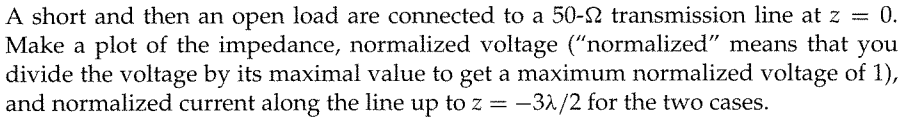
\includegraphics[width=14cm]{f1}
\end{center}
\end{figure}

While this line is short-circuited, the impedence can be seen in example 18.6 from the textbook:
\[
  Z(z)=jZ_0\tan(\beta \abs{z})
\]
We know that $Z=\frac{V}{I}$.  This means that the sinusoidal components of V and I must make a tangent.
The solution to this is:
\[
  V(z)=jZ_0I(0)\sin(\beta\abs{z})\text{, }I(z)=I(0)\cos(\beta\abs{z})
\]
We can plot this:

\begin{figure}[H]
\begin{center}
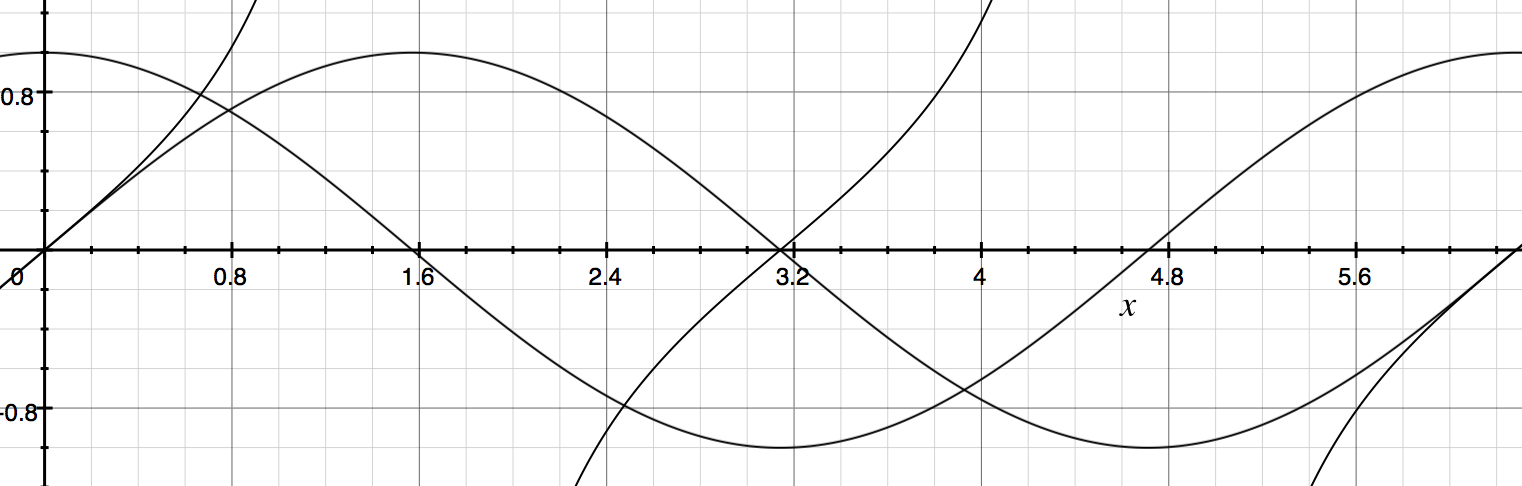
\includegraphics[width=14cm]{p1}
\end{center}
\end{figure}

The cosine curve is real, and the sine curve and tangent curve are imaginary.

Similarily, the textbook also tells us the loaded impedence and such:
\[
  Z(z)=\frac{Z_0}{j\tan(\beta\abs{z})}\text{, }V(z)=V(0)\cos(\beta\abs{z})\text{, }I(z)=\frac{jV(0)}{Z_0}\sin(\beta\abs{z})
\]

\begin{figure}[H]
\begin{center}
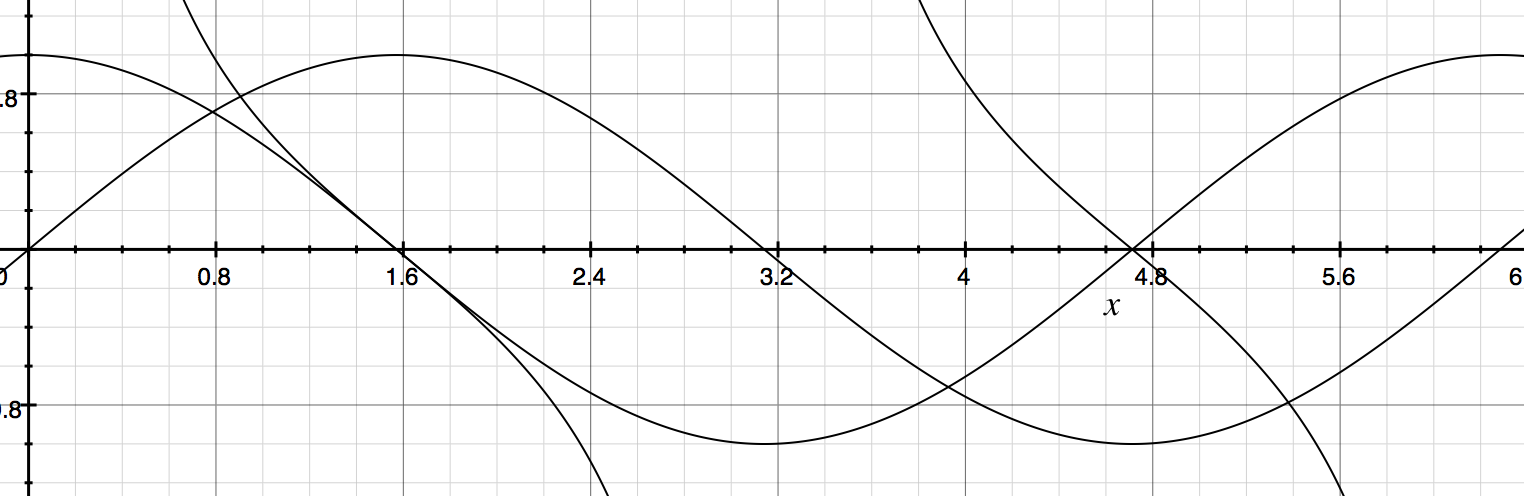
\includegraphics[width=14cm]{p2}
\end{center}
\end{figure}

only the cosine curve is real, the rest are imaginary.

2) \textbf{P18.10:}
\begin{figure}[H]
\begin{center}
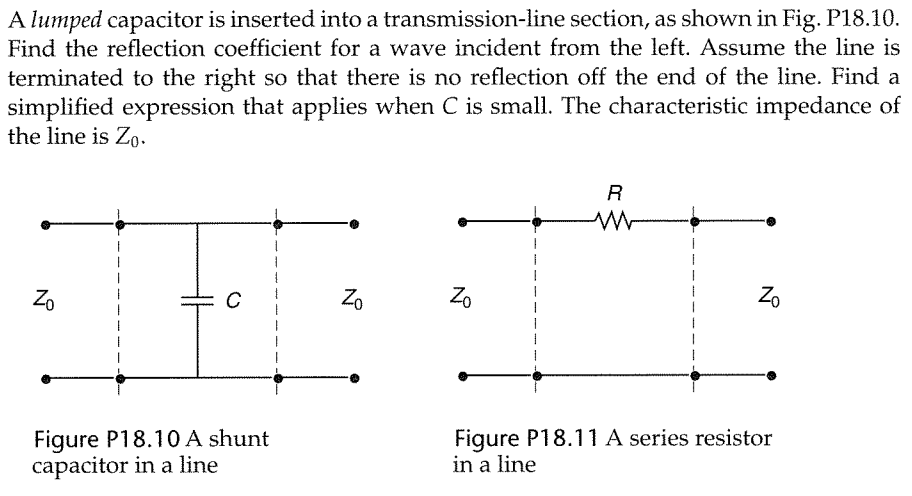
\includegraphics[width=14cm]{f2}
\end{center}
\end{figure}

The equivalent impedence
\[
  Z_e=\frac{Z_0/(1/j\omega C)}{Z_0+1/(j\omega C)} = \frac{Z_0}{1+j\omega C Z_0}
\]
This gives us the reflection coefficient
\[
  \rho = \frac{Z_e-Z_0}{Z_e+Z_0} = \frac{-j \omega CZ_0}{2+j\omega CZ_0} = -\frac{\omega^2C^2Z^2_0}{4+\omega^2C^2Z_0^2} - \frac{2j\omega CZ_0}{4+\omega^2C^2Z_0^2}
\]
When C is small
\[
  \rho \approx \frac{\omega CZ_0}{2j}
\]


3) \textbf{P18.12:}
\begin{figure}[H]
\begin{center}
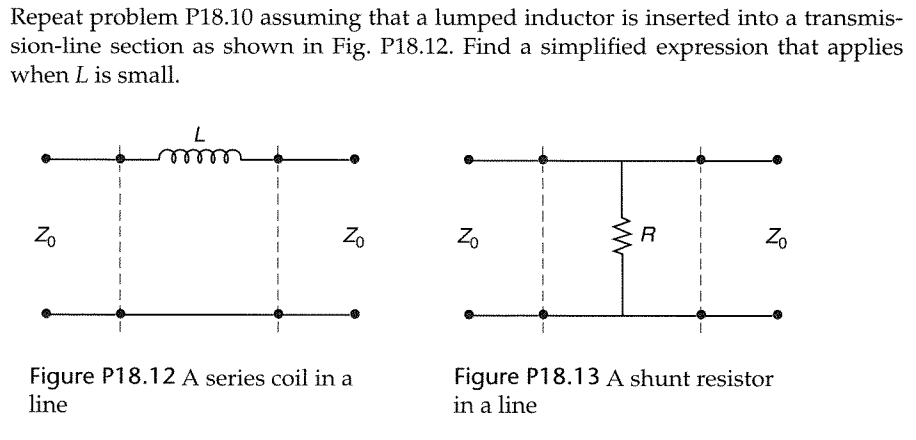
\includegraphics[width=14cm]{f3}
\end{center}
\end{figure}

The equivalent impedence
\[
  Z_e=Z_0+Lj\omega
\]
This gives us the reflection coefficient
\[
  \rho = \frac{Z_e-Z_0}{Z_e+Z_0} = \frac{Lj\omega}{Lj\omega+Z_0}
\]
When L is small:
\[
  \rho \approx \frac{Lj\omega}{Z_0}
\]

\newpage
4) \textbf{P18.17:}
\begin{figure}[H]
\begin{center}
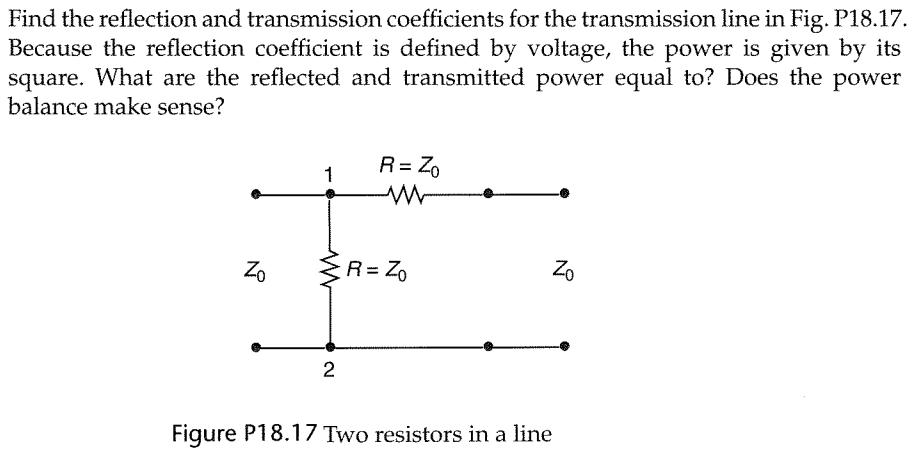
\includegraphics[width=13cm]{f4}
\end{center}
\end{figure}
This is a transmission line where $Z_e = \frac{2}{3}Z_0$.  We can for an equation:
\[
  \rho = \frac{\frac{-1}{3}Z_0}{\frac{5}{3}Z_0} = -0.2Z_0
\]
\[
  \tau = \rho+1 = 0.8Z_0
\]
This means that the power reflected is $0.04$ the power transmitted is $0.64$.  The
difference is the power loss through the impedence.

5) \textbf{P18.23:}
\begin{figure}[H]
\begin{center}
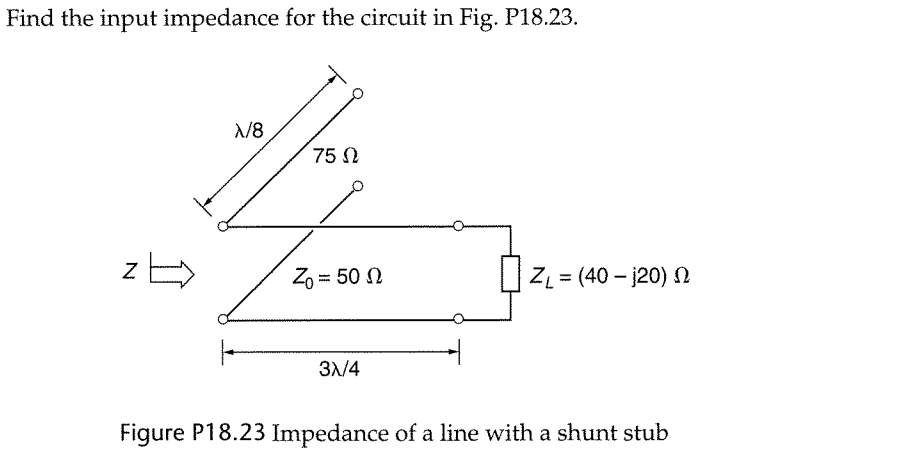
\includegraphics[width=14cm]{f5}
\end{center}
\end{figure}

We know the impedence to be:
\[
  Z=Z_0\frac{Z_L+jZ_0\tan(\beta\zeta)}{Z_0+jZ_L\tan(\beta\zeta)} = Z_0\frac{Z_L+jZ_0\tan(\frac{2\pi}{\lambda}\frac{3\lambda}{4})}{Z_0+jZ_L\tan(\frac{2\pi}{\lambda}\frac{3\lambda}{4})}
\]
\[
  = Z_0\frac{75+jZ_0\tan(\frac{3}{2})}{Z_0+j75\tan(\frac{3}{2})}
\]
6) \textbf{P18.24:}
\begin{figure}[H]
\begin{center}
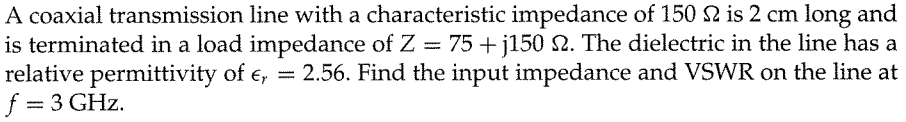
\includegraphics[width=14cm]{f6}
\end{center}
\end{figure}
We can find that the electrical length is $\zeta=\frac{2}{\lambda}=\frac{2}{10}=\frac{1}{5}$.  This
gives us the input impedence: ($\beta=\frac{\pi}{5}$)
\[
  Z=150\frac{75+j150+j(150)\tan(\pi/25)}{150+j(75+j150)\tan(\pi/25)}
\]
\[
  \rho=\frac{Z_L-Z_0}{Z_L+Z_0}=\frac{75+150j-150}{75+150j+150} = \frac{1+8j}{13}
\]
\[
  \text{VSWR }=-\frac{2+8i}{8i}=\frac{j}{4}-1
\]
7) \textbf{P18.31:}
\begin{figure}[H]
\begin{center}
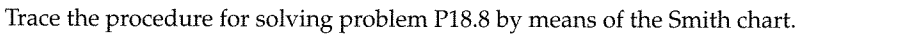
\includegraphics[width=14cm]{f7}
\end{center}
\end{figure}

the normalized load impedence of the first line $Z_{1L}=\frac{Z_l}{Z_{01}}$.  We begin at this point
then rotate wavelength clockwise by $\frac{\zeta_1}{\lambda}$.  The normalized impedance along the first
line is thus $z_1(\zeta_1)$ Which tells us the actual impedance $Z_1(\zeta_1)=Z_{01}z_1(\zeta_1)$.  We
then repeat this for line two, to find the new impedance $Z_2(\zeta_2)=Z_{02}z_2(\zeta_2)$.  Once we have the
impedance we can find the corresponding reflection coefficient.
\[
  \rho=\frac{Z_L-Z_1-Z_2}{Z_L+Z_1+Z_2}
\]
\[
  \text{VSWR }=\frac{1+\abs{\rho}}{1-\abs{\rho}}
\]

8) \textbf{P18.35:}
\begin{figure}[H]
\begin{center}
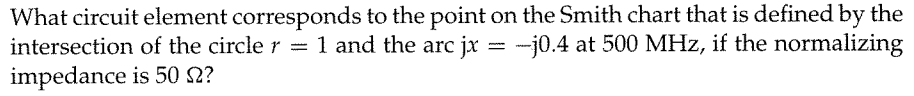
\includegraphics[width=14cm]{f8}
\end{center}
\end{figure}

This is going to be a combination of a negative imaginary part and a positive real part.  This is a resistor
in series capacitor.  The value of the resistor is the impedance, $50\Omega$.  The value of the capacitor
can be found:
\[
  C \Rightarrow \frac{1}{j2\pi500\cdot10^{6}C}=-0.4j
\]
\[
  \frac{1}{\pi*10^9C}=0.4 \Rightarrow C=318.3pF
\]

\end{document}
